\section{Forschungsplan}

Das Thema Netzwerksicherheit beinhalt viele Forschungsrichtungen, die zu umfangreich für eine einfache
Recherche sind. Aus diesem Grund und aus Knappheit von Platz konzentrierte sich diese Untersuchung auf zwei
spezifische Aspekte des Themas, und zwar auf Schwachstelle und auf Härtungsmaßnahmen von NFC und von Smartcards.
Diese Untersuchung wurde auch konzipert, indem folgende Methode benutzen wurden, um die vertrauenswürdigen
Daten zu sammeln:

\begin{itemize}
  \item Durchführung von Experimenten mit Smartcards und mit NFC
  \item Beobachtung von Angriffsmöglichkeiten
  \item Interview mit IT-SicherheitsFirmen
  \item Literaturrecherche
\end{itemize}

Der IT-Bereich entwickelte seine eigene Forschungsmethode mit Basis von anderen Fachrichtungen \cite{inbook:AHDS}.
Aus diesem Grund müssen sowohl die Recherche als auch ihre Darstellung so angepasst werden, sodass die Recherche selbst
und deren Ergebnis deutlich präsentiert werden können. Da Forschung und ihre Methode kein fester Bau darstellen, 
sind Flexibilität und Vielvaltigkeit der Quellen eine wichtige Voraussetzung für die Entwicklung eine erfolgreiche und
glaubwürdige Untersuchung.


Jedes Element dieser wissenschaftlichen Arbeit wurde so konzipert, sodass sie der Richtlinien von \cite{refip:SGRM} für 
die Entwicklung von Forschungen in dem IT-Bereich entsprechen. Die verwendten Methoden baten eine theoretische
und praktische Abbildung des Objekts dieser Untersuchung an, um ihre Anwendung direkt in der realen Welt darzustellen. 
Im Nachhinein werden die Durchführungsverfahren jeder Methode dieser Arbeit ausführlich beschrieben. Die folgende Abbildung 
zeigt zuerst den Rechercheweg dieser Untersuchung.

\begin{landscape}
  \thispagestyle{mylandscape}
  \begin{figure}[h]  
  \centering
    \centering{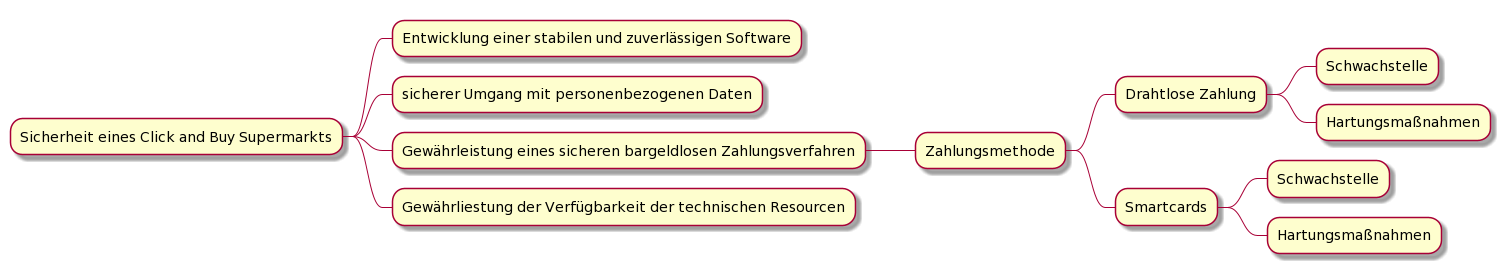
\includegraphics[width=20cm]{Bilder/Diagram2.png}}
         \caption{Recherchespfad (eigenes Bild)}
          \label{fig:diagramfrage}
  \end{figure}
\end{landscape}


\subsection{Experimenten mit Smartcards und mit NFC}
\textbf{Hier testen wir NFC und Smartcard vllt ohne und mit Hartungsmassnahmen, um zu zeigen, dass Massnahmen X gegen
Angriff Y geschützt ist}

\subsection{Beobachtung von Angriffsmöglichkeiten}
\textbf{Hier können wir sagen, dass wir in einem Labor einige Angriffe durchgeführt haben. Wir beschreiben alle Elementen
dieses Labor und was wir von diesem Experimenten erwarten. Auch die Quelle für solche Beobachtung.}

\subsection{Interview mit IT-SicherheitsFirmen}

\textbf{Hier schreiben wir, dass wir Person x der Firma y nach dem ihrem Produkt bezüglich auf Sicherheit gefragt haben.
Vllt. 9 Frage, 3 über das Produkt, 3 über Schwachstelle und 3 über Härtung. Wir brauchen auch am Anfang irgendwelche Zitation
wie eine wissenschaftliche Interview aussehen sollte.}

\subsection{Literaturrecherche}

Die Literatur bezüglich Netzwerksicherheit, bargeldlose Zahlungsverfahren und Vending Machines ist in den 
letzten 20 Jahren deutlich umfangreicher geworden. Da diese Begriffe viele und fast unendliche Konzepte 
decken, gehen wir hier auf spezifische Aspekte dieser Begriffe ein und zwar auf die Sicherheit von drahtlosen 
Zahlungsmethode und von Smartcards. 

Folgende Quelle trugen zu der Suchen nach vertrauenswürdigen Literaturquelle bei:

\begin{itemize}
    \item ScienceDirect
    \item Researchg Gate
    \item IEEE Xplore
    \item Google Scholar.
\end{itemize}

Diese Quellen ermöglichten ein allgemeines theoretisches Kenntnis über das Objekt dieser Untersuchung und dessen aktuellen 
Stand der Entwicklung.
